\section{Ziel}
In diesem Versuch soll die Verdampfungswärme L, ihre Temperaturabhängigkeit sowie die Dampfdruckkurve
von Wasser ebenso wie von einer anderen Substanz bestimmt werden.
\section{Theorie}
\label{sec:Theorie}
\cite{sample}
Einem Stoff kann in fast allen Kombinationen aus Druck $p$ und Temperatur $T$ eine feste Phase zugeorndet werden.
Im Allgemeinen wird zwischen den Phasen fest, flüssig und gasförmig unterschieden. Zwischen diesen Zuständen verlaufen jeweils
sogenannte Dampfdruckkurven. Wird sich auf einer dieser Kurven bewegt, koexistieren die zwei Zustände, welche sich jeweils neben der Kurve befinden.
Visualisiert  wird das ganze in einem Zustandsdiagramm. Ebenso sind die Punkte "TP" \, sowie "KP" wichtig zu erläutern. Der Tripelpunkt(TP) beschreibt jene Kombination
aus $p$ und $T$, an der alle drei Phasen koexistieren. Von ihm aus startet die, zwischen der gasförmigen und flüssigen Phase verlaufenden, Dampfdruckkurve und
endet am kritischen Punkt(KP). Entlängs dieser Kurve hat das System nur noch einen Freheitsgrad - $T$ -, da zu jeder Temperatur ein Druck festgelegt ist.
\begin{figure}[h]
    \centering
    \includegraphics[scale=0.8]{"screen.jpg"}
    \caption{Qualitatives Zustandsdiagramm des Wassers. Der Druck $p$ ist gegen die Temperatur $T$ aufgetragen.}
    \label{Abb1:Zustandsdiagramm}
\end{figure}
\noindent
Eine weitere, wichtig einzuführende Größe, ist die molare Verdampfungswärme $L$. Sie besitzt die Einheit $\unit{Joule/Mol}$ und beschreibt die Menge an Energie, um einen Mol
des Stoffes in einen gasförmigen Zustand zu bringen. Daher ist sie maßgebend für den Verlauf der Dampfdruckkurve. In unserem Messbereich
wird L als Konstante angenommen.\\
Aus der Thermodynamik ist bekannt, dass die Temperatur eines Stoffes über die gemittelte Stoßzeit eines Teilchens zur "Wand"\, oder mit anderen Teilchen definiert ist. Die Teilchen
mit der kürzesten mittleren Stoßzeit, sind auch jene mit der größten kinetischen Energie. Soll ein Stoff also zum verdampfen gebracht werden, muss ihm Energie zugeführt werden,
was wiederum die Teilchengeschwindigkeit erhöht. Hat ein Teilchen genug kinetische Energie, kann es aus der flüssigen (festen) Umgebung austreten - der Stoff verdampft. Für dieses Phänomen
braucht man genau die Energiemenge $L$. Das Austreten der Teilchen aus der Flüssigkeit (Festkörper) bewirkt ebenfalls einen Anstieg des Drucks im Gas oberhalb.\\
Nach langer Zeit stellt sich ein Gleichgewicht zwischen jenen Teilchen, welche die Flüssigkeit verlassen, und denen, die sich zurück in die Flüssigkeit bewegen, ein Gleichgewicht ein. Der so erreichte Druck im Dampf
wird mit Sättigungsdampfdruck bezeichnet. Dieser ist nicht abhängig vom Volumen in dem sich der Dampf befindet. Ändert sich dieses Volumen, wird nicht der Druck, sondern das Gleichgewicht verändert. Daher gilt die allgmein bekannte Gasgleichung
pV=RT nicht.\\
Im Folgenden soll eine Differentialgleichung bestimmt werden, welche zur Bestimmung der Dampfdruckkurve führt.
Dazu muss folgender Kreisprozess, für ein Mol, mathematisch näher betrachtet werden.
\begin{figure}[h!]
    \centering
    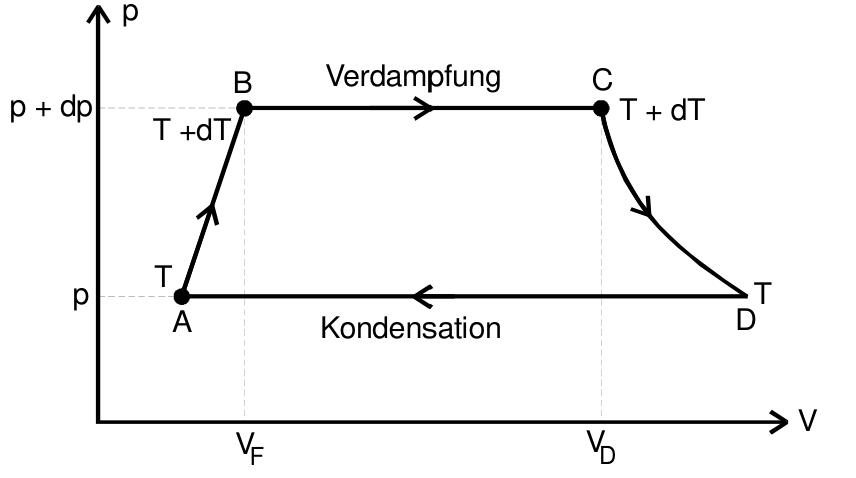
\includegraphics[scale=0.8]{sreen2.jpg}
    \caption{Kreisprozess für Verdampfung und Kondensation eines Stoffes. Der Druck p ist
    gegen das Volumen V dargestellt.}
    \label{Abb2:Kreisprozess}
\end{figure}
\\
Durch mathematische Überlegungen ergibt sich folgende Differentialgleichung:
\begin{equation}
    (V_D-V_F)dp=\frac{L}{T}dT
\end{equation}
Diese Differentialgleichung trägt den Namen Clausius-Clapeyronsche Gleichung.
Auf beiden Seiten des Gleichheitszeichens stehen Ausdrücke für die gesamt
geleistete Arbeit, die sich links aus der Volumendifferenz von B zu C sowie einer infitisimalen
Druckänderung ergibt.
Rechts beschreibt der Quotient der Verdampfungswärme mit der Temperatur um eine infitisimal kleine
Temperaturänderung die Gesamtarbeit.\\
Unter der Bedingung, dass $V_D$, $V_F$ und $L$ konstant seien, ist diese Gleichung gut lösbar. Dies ist im
Allgemeinen jedoch nur in manchen Temperaturbereichen möglich. Hier wird der Fall behandelt, dass $T$ deutlich kleiner
als die kritische Temperatur $T_\text{Kr}$ ist.
\newpage
Somit sind folgende Annahmen zu treffen:
\begin{itemize}
    \item[1.] $V_F<<V_D$. Daher darf $V_F$ vernachlässigt werden.
    \item[2.] Für $V_D$ gilt die ideale Gasgleichung: $V_D(p,T)=\frac{T}{p}$
    \item[3.] L darf keine Abhängigkeit von Druck $p$ oder Temperatur $T$ haben. Damit
    ergibt sich als Lösung der DGL: $p=p_0\cdot \exp(-\frac{1}{T}\cdot\frac{L}{R})$
\end{itemize}
Es existiert also eine Proportionalität zwischen der Molekühlanzahl in der Damfphase sowie
des Drucks oberhalb der Flüssigkeit. Wie vorhin diskutiert, braucht ein Teilchen jedoch eine gewisse
kinetische Energie zum Austreteten aus der Flüssigkeit, was durch die Boltzmann-Statistik parametrisiert wird.
Mit Gesamtenergie $W$ ergibt sich für den Bruchteil der Moleküle, die austreten könnten:
$\exp(-W/kT)\Rightarrow p\propto \exp(-W/kT)$.
\begin{figure}
    \centering
    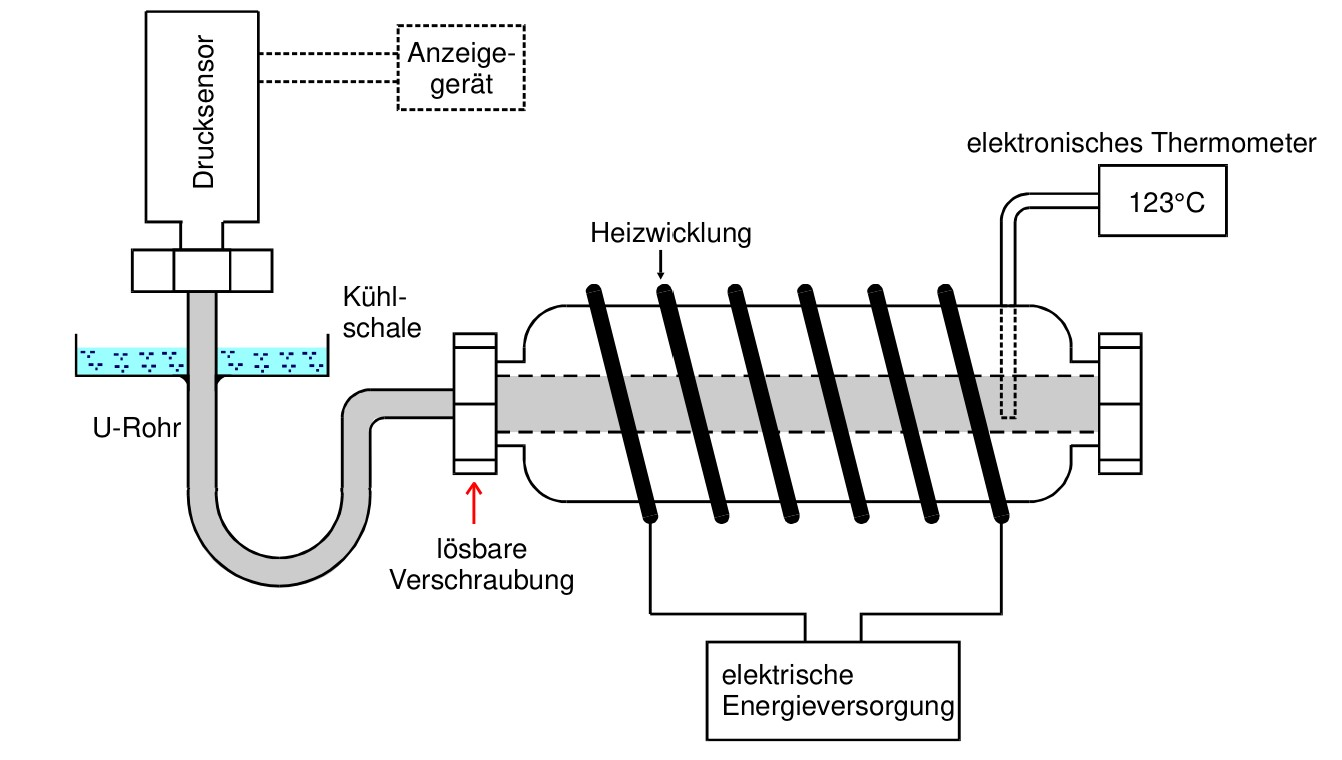
\includegraphics[scale=0.6]{screen3.jpg}
\end{figure}
